%%7:1:0 23/4/2019%%5:30:29 23/4/2019 -VieTeX creates C:\Users\Administrator\Desktop\.tex
% LaTeX Book Template - using defaults
\documentclass[12pt,a4paper]{book}
\usepackage{amsmath,amsxtra,amssymb,latexsym, amscd,amsthm}
\usepackage{indentfirst}
\usepackage[mathscr]{eucal}
\usepackage{color}
\usepackage[utf8]{vietnam}
\usepackage{graphicx}
\usepackage[left=2.5cm,right=3cm,top=3cm,bottom=3cm]{geometry}
\newtheorem{note}{Chú ý}
\newtheorem{dn}{Định nghĩa}
\newtheorem{md}{Mệnh đề}
\newtheorem{dl}{Định lý}
\newtheorem{bd}{Bổ đề}
\newtheorem{vd}{Ví dụ}
\newtheorem{hq}{Hệ quả}
\newtheorem{op}{Trường hợp}
\newtheorem{al}{Thuật toán}
\def\tSi{\tilde{\Sigma}}
\newcommand{\m}[1]{
\begin{bmatrix}
#1
\end{bmatrix}
}

% Set the beginning of a LaTeX document
\begin{document}
\title{VỀ HÀM LAMBERT VÀ ỨNG DỤNG CHO CÁC PHƯƠNG TRÌNH VI PHÂN CÓ TRỄ}         
\author{Lê Tiến Lượng \\ K61A1T - Đại học khoa học tự nhiên Hà Nội \\ Giảng viên hướng dẫn : TS. Hà Phi}        
\date{15/05/2019}       
\maketitle
\tableofcontents %Muc luc
		 %end Muc luc
	
	\chapter{Giới thiệu hàm Lambert}
	\section{Giới thiệu}       
		Hàm Lambert $W$ được định nghĩa là một hàm phức ngược đa trị của hàm $w \mapsto we^{w}$ với $w \in \mathbb{C}$. Hàm này có rất nhiều ứng dụng trong cả toán thuần túy và toán ứng dụng và một trong số chúng sẽ được trình bày trong mục 2.2 dưới đây. \\    
		Năm 1758, Lambert nghiên cứu phương trình $x = q + x^{m}$ với ẩn số x. Trong [1], Euler biến đổi phương trình Lambert về dạng đối xứng hơn \begin{align}x^{\alpha} - x^{\beta} = (\alpha - \beta)vx^{\alpha + \beta} \end{align}
 bởi thay thế $x = x^{-\beta}$ và đặt $m = \frac{\alpha}{\beta}$ và $q = (\alpha - \beta)v$.
		Phiên bản Euler của chuỗi Lambert có dạng sau 
		\begin{align}
			\begin{split}
				x^{\gamma} = 1 + \gamma v + \frac{1}{2}\gamma(\gamma + \alpha + \beta)v^{2} + \frac{1}{6}\gamma(\gamma + \alpha + 2\beta)(\gamma + 2\alpha + \beta)v^{3} \\ + \frac{1}{24}\gamma(\gamma + \alpha + 3\beta)(\gamma + 2\alpha + 2\beta)(\gamma + 3\alpha + \beta)v^{4} + ...
			\end{split}
		\end{align}
	Sau khi chuyển đổi chuỗi, Euler nhìn vào trường hợp đặc biệt, bắt đầu từ $\alpha = \beta$. Để nhìn thấy ý tưởng từ phương trình ban đầu, ta chia (1.1) cho $(\alpha - \beta)$ và cho $\beta \rightarrow \alpha$, ta được
		\begin{align*}
			\displaystyle \lim_{\beta \to \alpha}\frac{x^{\alpha}-x^{\beta}}{\alpha - \beta} = vx^{2\alpha}\\
			\mbox{Do đó } x^{\alpha}\log \alpha = vx^{2\alpha}
		\end{align*}
		\begin{align}
			\mbox{Vì vậy } \log x = vx^{\alpha}
		\end{align}
	Euler chú ý rằng nếu chúng ta giải được phương trình (1.3) với $\alpha = 1$ thì chúng ta có thể giải được nó với mọi $\alpha \neq 0$. Để thấy điều này,ta nhân phương trình (1.3) với $\alpha$,dẫn đến $\alpha \log x = \log x^{\alpha}$. Đặt $z = x^{\alpha}$ và $u = \alpha v$, ta có $\log z = u z$ là kết quả phương trình (1.3) với $\alpha = 1$. \\
	Để giải phương trình (1.2), đầu tiên Euler cho $\alpha = \beta = 1$ và viết lại (1.2) dưới dạng chuỗi của $\frac{x^{\gamma}-1}{\gamma}$. Từ phương trình (1.2) thì 
		\begin{align*}
			\frac{x^{\gamma}-1}{\gamma} = v + \frac{1}{2}(\gamma+2)v^{2} + \frac{1}{6}(\gamma+3)(\gamma+3)v^{3} + ... 
		\end{align*}
		Tiếp đến, ông cho $\gamma \rightarrow$ 0, vì \begin{align*} \displaystyle \lim_{\gamma \to 0}\frac{x^{\gamma}-1}{\gamma} = \log x 
		\end{align*}
		\begin{align} \mbox{nên ta thu được }\log x = v + \frac{2^{1}}{2!}v^{2} + \frac{3^{2}}{3!}v^{3} + \frac{4^3}{4!}v^{4} + ... 
		\end{align}
		Chuỗi này hội tụ với $|v| < \frac{1}{e}$,nó được định nghĩa là hàm $T(v)$ gọi là hàm cây [2]. Nó có giá trị bằng với $-W(-v)$ với $W(z)$ được định nghĩa là hàm thỏa mãn 
		\begin{align}
			W(z)e^{W(z)} = z.
		\end{align} 
		Chúng ta sẽ gọi tắt 2 hàm này là $T$ và $W$. Hai hàm này được sử dụng trong rất nhiều ứng dụng như : liệt kê số cây $[3,4]$, tính toán độ cao cột nước $[5]$ và trong bài toán được xem xét bởi Pólya và Szego $[6]$.Wright sử dụng nhánh phức của hàm $W$ và tính tổng quát của hàm mũ để tính toán phương trình vi phân có trễ hệ số hằng.\\
		Hàm Lambert $W$ là hàm có giá trị phức tạp, cùng với đối số phức tạp $z$ và nó có vô hạn nhánh $W_{k}$, ở đó $k = -\infty, ..., -1, 0 , 1, \infty$. Đường thẳng thực của nhánh chính của hàm Lambert $W$ ,$W_{0}$ có giá trị nhỏ nhất là -1. Nhánh chính và tất cả các nhánh khác của hàm Lambert có thể được tính toán giải tích thông qua việc tính toán chuỗi. Các ngôn ngữ tính toán khoa học phổ biến hiện nay như Python, Matlab, Maple, Mathematica, ... đều có hàm Lambert (vô hướng) dựng sẵn với độ chính xác tùy ý.
\begin{verbatim}
syms x
fplot(lambertw(x))
hold on
fplot(lambertw(-1,x))
hold off
axis([-0.5 4 -4 2])
title('Hàm Lambert W , 2 nhánh chính')
legend('k=0','k=-1','Location','best')
\end{verbatim}
\begin{figure}
    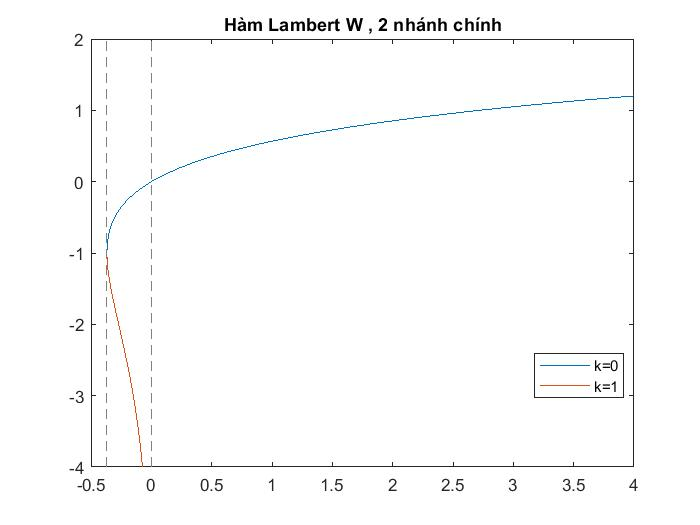
\includegraphics[scale=0.5]{wfig.jpg}
    \caption{Hàm Lambert với 2 nhánh chính k=0, k=-1}
\end{figure}


	\section{Các tính chất của hàm Lambert}
	Chúng ta sẽ bắt đầu bằng việc xác định miền hội tụ của nhánh chính $W_{0}(x)$ được biểu diễn dưới dạng chuỗi lũy thừa theo định lý Larange như sau \\
	Giả sử z được định nghĩa là hàm của x theo phương trình có dạng $z = f(x)$\\
trong đó $f$ là giải tích tại $x_0$ và $f'(x_{0}) \neq 0$. Từ đó ta có thể đảo ngược hay giải phương trình với $x = g(z)$ bằng chuỗi lũy thừa. 
\begin{align}
g(z) &= x_0 + \displaystyle \sum_{n=1}^{\infty}g_n \frac{(z-f(x_0))^{n}}{n!}) \notag \\
\mbox{với }g_n &= \displaystyle \lim_{x \to x_0} \left[\frac{d^{n-1}}{dx^{n-1}}\left(\frac{x-x_0}{f(x)-f(x_0)}\right)^{n}\right]
\end{align}
Áp dụng định lý Larange, ta có khai triển chuỗi của nhánh $W_0(z)$ là $W_0(z) = \displaystyle \sum_{n=1}^{\infty}\frac{(-n)^{n-1}}{n!}z^{n}$\\
Thật vậy, đặt $f(x) = xe^{x}$ ,chọn $x_0 = 0 \mbox{ do đó } f(x_0) = 0$. Khi đó $f'(x) = e^{x} + xe^{x} \mbox{ do đó } f'(x_0) = 1$.
\begin{align*}
W_{0}(z) &= \displaystyle \sum_{n=1}^{\infty}g_n\frac{z^{n}}{n!} \\
\mbox{với }g_n &= \displaystyle \lim_{x \rightarrow 0}\frac{d^{n-1}}{dx^{n-1}}\frac{x^{n}}{f^{n}x}
=  \displaystyle \lim_{x \rightarrow 0}\frac{d^{n-1}}{dx^{n-1}}(\frac{x}{xe^{x}})^{n} 
= \displaystyle \lim_{x \rightarrow 0}\frac{d^{n-1}}{dx^{n-1}}e^{-nx} = \displaystyle \lim_{x \rightarrow 0}(-n)^{n-1}e^{-nx} \\
&= (-n)^{n-1}
\end{align*}

Vì vậy
\begin{align*}
W_0(z) = \displaystyle \sum_{n=1}^{\infty}\frac{(-n)^{n-1}}{n!}z^{n}
\end{align*}
Theo tiêu chuẩn D' Alembert thì chuỗi lũy thừa $\displaystyle \sum_{n=0}^{\infty}(a_nz^{n})$ có bán kính hội tụ là  \\
r = $\displaystyle \lim_{x \to \infty}\frac{|a_n|}{|a_{n+1}|}$ \\
Áp dụng tiêu chuẩn D'Alembert vào chuỗi $W_0(z) = \displaystyle \sum_{n=1}^{\infty}\frac{(-n)^{n-1}}{n!}z^{n}$ \\
Đặt $a_n =\frac{n^{n-1}}{n!} \mbox{ ta có } \frac{a_n}{a_{n+1}} = \frac{n^{n-1}}{n!} \Bigg/ \frac{(n+1)^{n}}{(n+1)!} \\
= \frac{1}{(\frac{n+1}{n})^{n-1}} = \frac{1}{(1+\frac{1}{n})^{n-1}} \xrightarrow{n \rightarrow \infty} \frac{1}{e}\\
\mbox{Do đó }r = \displaystyle \lim_{n \to \infty}\frac{|a_n|}{|a_{n+1}|} = \frac{1}{e}$.
Vậy bán kính hội tụ của chuỗi $W_0(z)$ là $\frac{1}{e}$.
Nói về sự hội tụ này , Euler đã không chỉ ra rằng chuỗi (1.2) hội tụ với 
\begin{align*}
	M_E(\alpha,\beta)|v| < \frac{1}{e}
\end{align*}
trong đó $M_E(a,b) = \sqrt{\frac{a^2+b^2}{2}}$ \\
Xét hàm Lambert $W(x)$ thỏa mãn $x = W(x)e^{W(x)}$, ta đi tìm $W'(x)$:
Tại mọi điểm mà $W$ là khả vi, ta sẽ có 
\begin{align}
\frac{d}{dx}W(x)e^{W(x)} &= \frac{dx}{dx} &= 1 \nonumber \\  
\mbox{Do đó }W'(x)e^{W(x)} + W(x)W'(x)e^{W(x)} = W'(x)e^{W(x)}(1+W(x)) \tag{*}\\
\mbox{Vì vậy } W'(x) = \frac{1}{e^{W(x)}(1+W(x))} = \frac{W(x)}{x(1+W(x))} ,\mbox{ với mọi } x \neq 0, x \neq \frac{-1}{e} \nonumber
\end{align}
Ngoài ra, nếu ta xét nhánh chính $W_{0}$ và $x=0$ thì từ $(*)$ ta có $1 = W'(0)e^{W(0)}(1+W(0)) = W'(0)e^{0}(1+0)$ \\
Do đó $W'_{0}(0) = 1$.
Nói thêm về đạo hàm, chúng ta sẽ dùng phương pháp quy nạp để tính đạo hàm cấp $n$ của $W$ với $n \ge 1$ là 
$$ \frac{d^{n}W(x)}{dx^n} = \frac{e^{-nW(x)}p_n(W(x))}{(1+W(x))^{2n-1}},$$ với $n \ge 1 $ \\
trong đó đa thức $p_n(w)$ thỏa mãn ràng buộc :\\
$$ p_{n+1}(w) = -(nw + 3n - 1)p_n(w) + (1+w)p'_n(w), $$ \\
Về công thức chi tiết và các tính toán của $p_n$ và $p'_n$, xem tài liệu $[7,8]$ \\
Ta có công thức sau đối với nhánh chính khi $z = We^{W} > 0 $
$$ \log W(z) = \log z - W(z) $$ xem $[9]$ để biết thêm công thức tổng quát.
Bây giờ, chúng ta sẽ trả lời câu hỏi về việc tính tích phân các biểu thức chứa hàm Lambert W. Trong [10], K. B. Ranger sử dụng bài tập để minh họa việc tính tích phân của phương trình Navier-Stokes trong dạng tham số 
\begin{align}
 x = pe^{p},\\
\frac{dy}{dx} = p. \\
\Rightarrow \frac{dx}{dy} = \frac{d(pe^{p})}{dy} = \frac{dp}{dy}pe^{p} + \frac{dp}{dy}e^{p} = e^{p}\frac{dp}{dy}(1+p) = \frac{1}{p} \nonumber \\
\Rightarrow \frac{dy}{dp} = p(p+1)e^{p} 
\end{align}
Từ phương trình (1.9)ta có thể dễ dàng lấy tích phân để thu được : \\
$$ y = (p^{2} - p + 1)e^{p}  +  C $$\\
Vì $y$ là nguyên hàm của $W(x)$, Ranger đã phát hiện ra một phương pháp đơn giản để tính tích phân của $W(x)$ như sau 
$$ \displaystyle \int(W(x)dx) = (W^2(x) - W(x) +1)e^{W(x)} + C  \\
= x(W(x) - 1 + \frac{1}{W(x)}) + C $$
Khi ta thử kỹ thuật này trên các hàm khác có chứa W, ta thấy rằng đó là sự thay đổi đặc biệt của biến. Đặt $w = W(x)$, do đó $x = we^w$ và $dx = (w+1)e^{w}dw$
\begin{align*}
\displaystyle \int{xW(x)dx} &= \displaystyle \int{we^{w}.w.(1+w)e^{w}dw} \\
&= \frac{1}{8}(2w-1)(2w^{2}+1)e^{2w} + C  \\
&= \frac{1}{2}(W(x)-\frac{1}{2})(W^{2}(x)+\frac{1}{2})e^{2W(x)} + C
\end{align*}
Điều này đúng cho mọi nhánh của W, theo định nghĩa $\frac{d}{dw}we^{w} \neq 0$ tại điểm trong bất kỳ thuộc nhánh bất kỳ. \\
Bài toán tích phân của các biểu thức chứa $W$ là trường hợp đặc biệt của phép lấy tích phân các biểu thức của hàm ngược. Bằng việc sử dụng kỹ thuật đã nêu trên thì chúng ta có công thức sau, xem thêm tại $[10]$
\begin{align*}
\displaystyle \int{f^{-1}(x)dx} = yf(y) -\displaystyle \int{f(y)dy}
\end{align*}
Thật vậy, đặt $x = f(y)$ \\
$\mbox{Do đó } \displaystyle \int{f^{-1}(x)dx} = \displaystyle \int{ydf(y)} = yf(y) - \displaystyle \int{f(y)dy} + C $ \\
Cuối cùng, lưu ý rằng kỹ thuật này cho phép thuật toán Risch được áp dụng để xác định tích phân có chứa $W$ có phải là sơ cấp hay không. Xem thêm thuật toán Risch tại $[11]$
\section{Một số ứng dụng của hàm Lambert}
\subsection{Bài toán về mô hình đốt cháy}
 Bài toán 
$$ \frac{dy}{dt} = y^{2}(1-y),\quad y(0) = \varepsilon > 0 $$ được sử dụng trong $[12,17]$ để nghiên cứu phương pháp nhiễu. Ta chỉ công thức nghiệm hiển theo hàm $W$, và do đó mọi kết quả nhiễu trong $[12]$ có thể được kiểm chứng lại bằng cách so sánh với nghiệm chính xác. Bài toán mô hình là phương trình phân ly biến số và tích phân sẽ cho kết quả là dạng ẩn của $y(t)$ như sau
\begin{align*} \frac{1}{y} + \log (\frac{1}{y} -1 ) &= \frac{1}{\varepsilon} + \log (\frac{1}{\varepsilon}  - 1) - t  \\
\mbox{Do đó } e^{\frac{1}{y}}(\frac{1}{y} - 1) &= e^{\frac{1}{\varepsilon}-t}(\frac{1}{\varepsilon}-1)  \\
\mbox{Vì vậy } e^{\frac{1}{y}-1}(\frac{1}{y}-1) &= e^{\frac{1}{\varepsilon}-1-t}(\frac{1}{\varepsilon}-1) 
\end{align*}
Đặt $\frac{1}{\varepsilon} - 1 = u \mbox{ ta có } \frac{1}{y} - 1 = W(ue^{u-y}) \mbox{ do đó } y = \frac{1}{1+W(ue^{u-t})}$. Qua việc định tính phương trình vi phân,ta có thể chỉ ra rằng $0 < \varepsilon \le y < 1$, điều này chỉ ra rằng nhánh chính của hàm Lambert W cần được sử dụng. Bắt nguồn từ nghiệm hiển, tất cả các dạng chuỗi kết quả của hàm trong $[12]$ có thể dễ dàng được kiểm tra.
\subsection{Phương trình vi phân hệ số hằng}
Ví dụ cho dạng đơn giản của phương trình vi phân có trễ :
$$ \dot{y}(t) = ay(t-1), $$ với $y(t) = f(t)$ là 1 hàm đã biết , trên đoạn $0 \le t \le 1$. Ý nghĩa của bài toán bắt nguồn từ việc nghiên cứu sự ổn định của phương trình vi phân phi tuyến có trễ\\
Một cách tiếp cận bài toán là phỏng đoán y = $e^{st}$ là nghiệm với vài giá trị của s. Điều đó cho ta
$$ se^{st} = ae^{st}e^{-s} \\ \Rightarrow se^{s} = a $$ hay $$ s =  W_k(a) , $$  với nhánh bất kỳ $W_k$. 
Nếu $e^{W_k(a)t}$ là nghiệm của $ \dot{y} = ay(t-1) $ thì theo nguyên lý chồng chất nghiệm
$$ y = \displaystyle \sum_{k=-\infty}^{\infty}{c_ke^{W_k(a)t}}$$ cũng là nghiệm với mọi cách chọn $c_k$ "chấp nhận được".  Người ta thấy rằng nghiệm sẽ tăng theo cấp số mũ nếu một $W_k(a)$ nào đó có phần thực dương, và điều đó dẫn đến những định lý quan trọng trong lý thuyết của phương trình vi phân có trễ.\\
Cách tiếp cận này có thể được tổng quát hóa để nghiên cứu các phương trình vi phân có trễ hệ số hằng có dạng vô hướng
$$ \dot{y}(t) = ay(t-1) + by(t), $$ 
hoặc $ \dot{y} = Ay(t-1) + By(t)$ với $A, B$ là các ma trận giao hoán. Xem thêm $[18,19,20]$ về vấn đề này.
 

	\chapter{Hàm Lambert và phổ của phương trình vi phân có trễ}
\section{Giới thiệu}
Trong chương này, chúng ta sẽ xem xét các phương trình vi phân có trễ dạng sau :
\begin{align}
\sum = \begin{cases}
\dot{x}(t) &= Ax(t) + Bx(t-\tau), t > 0\\
x(t) &= \varphi(t) , t \in [-\varphi,0] \\
\end{cases} 
\end{align}
với $A, B  \in \mathbb{C}^{n \times n}$, trễ $\tau$ > 0. Phương trình đặc trưng tương ứng là
$$ 0 = \det (-sI + A + Be^{-s\tau}) \\$$
Ở đây, ta sẽ kí hiệu tập hợp tất cả các nghiệm  của phương trình đặc trưng(tập các giá trị riêng hay phổ) của $\sum$ bởi $\sigma_{\sum}$. \\
Không giống như phương trình vi phân không trễ, phương trình vi phân có trễ sẽ có vô hạn nhưng đếm được số giá trị riêng. Đó là một điểm khó khăn của phương trình vi phân có trễ từ quan điểm tính toán. Trong tài liệu, có một số kết quả về tính chất định tính của phổ. Ví dụ, chúng ta biết từ $[21]$ rằng giá trị riêng sẽ phân bố dọc theo các đường cong trong mặt phẳng phức (được gọi là xích các nghiệm) và với bất kỳ đường thẳng nào trong mặt phẳng phức thì chỉ có một số hữu hạn các giá trị riêng nằm bên phải của đường thẳng này.\\
Trong chương này, chúng ta sẽ nghiên cứu biểu diễn hiển của các giá trị riêng của lớp đặc biệt các phương trình vi phân có trễ dựa trên dạng ma trận của hàm Lambert $W$. Phổ của các hệ một trễ vô hướng có thể được tính toán sử dụng hàm Lambert, điều này đã được biết đến từ lâu, ví dụ như trong $[22]$. Trong $[23]$ và các nghiên cứu tiếp theo $[24]$ và $[25]$ thì những mở rộng cho trường hợp nhiều chiều sử dụng dạng ma trận của hàm Lambert $W$. Tuy nhiên các kết quả trong $[23]$ không đúng trong trường hợp tổng quát. Mục tiêu của chương này là đưa ra các điều kiện đủ cho các ma trận của hệ để công thức trong $[23]$ đúng. Cá biệt thì chúng ta sẽ chỉ ra rằng công thức là đúng nếu $A$ và $B$ là tam giác hóa được đồng thời. Những quan sát tương tự đã được nêu ra trong $[26]$ và hoàn toàn độc lập với nghiên cứu này, trong đó các kết quả gần tương tự nhận được không sử dụng công thức hiển cho hàm Lambert $W$. Ở đây chúng ta sẽ thiết lập các kết quả này cho các biểu diễn trong $[23]$. Hơn nữa, chúng ta sẽ trình bày các phản ví dụ, điều này chứng minh rằng công thức có thể sai. Điều này rất quan trọng vì kết quả của $[23]$ rất được quan điểm và được trích dẫn. Do đó đáng để làm rõ phạm vi ứng dụng của công thức.
\section{Dạng ma trận của hàm Lambert}
Nhắc lại rằng với z $\in \mathbb{C}$, hàm Lambert W được định nghĩa (đa trị) là hàm ngược của hàm $z \mapsto ze^{z}$ :
$$ W_k(z) \in \left\{w \in \mathbb{C} : z = we^{w}\right\}, $$ \\
trong đó $W_{k}$ là nhánh chính thứ $k, k \in \mathbb{Z}$ \\
Ngoài điểm $ z = -e^{-1}$ mà nhánh chính $W_0$ không khả vi, tại đó tất cả các nhánh đều là giải tích địa phương. Do đó, chúng ta định nghĩa hàm Lambert $W$ một cách tiêu chuẩn ví dụ như trong $[27]$ và $[28]$. Đầu tiên chúng ta định nghĩa hàm Lambert $W$ cho ma trận theo dạng chuẩn tắc Jordan
$$ J = diag (J_{n_{1}}(\lambda_{1}),J_{n_{2}}(\lambda_{2}),...,J_{n_{s}}(\lambda_{s})) $$
với $J_n(\lambda)$ là ma trận Jordan cỡ n $\times$ n tương ứng với giá trị riêng  $\lambda$ bội n.
Vậy :
$$ W_k(J) = diag (W_{k_{1}}(J_{n_{1}}(\lambda_{1})),W_{k_{2}}(J_{n_{2}}(\lambda_{2})),...,W_{k_{s}}(J_{n_{s}}(\lambda_{s}))).$$ \\
Chú ý rằng chúng ta được phép lấy các nhánh khác nhau cho mỗi khối Jordan. Nếu J có $s$ khối Jordan  và tập chỉ số cho các nhánh của hàm Lambert W là $\mathbb{Z}$ thì tập chỉ số của các nhánh $W_k(j)$ là $ \mathbb{Z}^{s} $  . \\
Với khối Jordan có số chiều là 1 thì ta có thể sử dụng hàm Lambert $W$ vô hướng . Với khối số chiều lớn hơn, ta sẽ định nghĩa hàm Lambert $W$ (với nhánh cố định) của một khối Jordan bởi định nghĩa tiêu chuẩn của hàm ma trận dạng
$$ P(J_k(\lambda)) = \left(
\begin{array}{cccc}
p(\lambda) & p'(\lambda) & \cdots & \frac{1}{(k-1)!}p^{(k-1)}(\lambda) \\
 & p(\lambda) & \ddots & \vdots \\
\vdots &  &\ddots & p'(\lambda) \\
 &  & \cdots & p(\lambda) \\
\end{array}
\right)
 \\ $$
$$ \Rightarrow W_k(J_n(\lambda)) =  \left(
\begin{array}{cccc}
W_k(\lambda) & W_k'(\lambda) & \cdots & \frac{1}{(n-1)!}W_{k}^{(n-1)}(\lambda) \\
 & W_k(\lambda) & \ddots & \vdots \\
\vdots &  &\ddots & W'_k(\lambda) \\
 &  & \cdots & W_k(\lambda) \\
\end{array}
\right) \\ $$
Nếu k = 0 thì ta phải giả sử thêm là $\lambda \neq -e^{-1}$(vì $W'_{0}(-e^{-1})$ không xác định). \\
Ta hoàn thành việc định nghĩa hàm Lambert W cho ma trận, bằng việc chuyển đổi ma trận về dạng chuẩn Jordan $A = SJS^{-1}$. Từ đó ta có thể định nghĩa
$$ W_k(A) = S W_k(J) S^{-1} $$
Với nhánh chính k = 0, từ bây giờ chúng ta sẽ giả sử rằng $-e^{-1}$ không phải là giá trị riêng tương ứng với khối Jordan với số chiều lớn hơn 1, tức là
\begin{align} rank (A + e^{-1}I) = rank (A + e^{-1}I)^{2} \end{align}
\begin{note} 
Giả thiết (3.2) làm giảm đi sự đẹp đẽ của hàm Lambert W. Điểm này được chỉ ra bởi Robert Corless.
\end{note}
\begin{vd}
Chúng ta sẽ minh họa định nghĩa hàm Lambert $W$ cho khối Jordan 2 $\times$ 2 với $\lambda \neq -e^{-1} : \\ $ 
\end{vd}
Cho
\begin{align*}
 J = \begin{bmatrix} 
\lambda & 1 \\
0 & \lambda
 \end{bmatrix} 
\end{align*}
thì 
\begin{align*}
 W_k(J) = \begin{bmatrix} 
W_k(\lambda) & W'_k(\lambda) \\
0 & W_k(\lambda) \end{bmatrix} 
\end{align*}
Chúng ta kiểm tra rằng $J = W_k(J)e^{W_k(J)}$ như sau. Vì $\lambda = W_k(\lambda)e^{W_k(\lambda)}$ ta có $1 = W'_k(\lambda)e^{W_k(\lambda )} + W'_k(\lambda)\lambda$
\begin{align*}
\mbox{Do đó } W_k(J)e^{W_k(J)} = \begin{bmatrix} 
W_k(\lambda) & W'_k(\lambda) \\
0 & W_k(\lambda) 
\end{bmatrix}
e^{W_k(\lambda)} \begin{bmatrix} 
1 & W'_k(\lambda) \\
0 & 1 
\end{bmatrix} \\
= \begin{bmatrix} 
\lambda & \lambda W'_k(\lambda) + e^{W_k(\lambda)} W'_k(\lambda)\\
0 & \lambda 
\end{bmatrix} 
 = J \\
\end{align*}
Mặt khác, nếu $\lambda = -e^{-1}$ thì $W_0(\lambda) = -1$ và giả thiết $W = \begin{bmatrix} 
-1 & w \\
0 & -1
\end{bmatrix}$ thì ta có $We^{W} = -e^{-1}I \mbox{ với mọi }  w \in \mathbb{C}$.Do đó, $\sigma(W) =  \left\{-1\right\}$ dẫn đến $We^{W} = -e^{-1}I$. Chúng ta kết luận rằng $W_0(J)$ không xác định trong trường hợp này vì $W_0(-e^{-1})$ không phải là duy nhất.
\section{Kết quả chính}
Sau đây chúng ta sẽ đi nghiên cứu công thức phổ cho các hệ phương trình vi phân có trễ trong một số trường hợp đặc biệt
 \begin{bd}
 Nếu $M = [m_{ij}]_{i,j = 1,...,n} \in \mathbb{R}^{n \times n}$ có dạng tam giác dưới hoặc tam giác trên thì dạng chuẩn tắc Jordan của M là $J_{M}$ sẽ chứa chính xác $m_{11}, ..., m_{nn}$ trên đường chéo chính (theo một hoán vị nào đó) \\
 \end{bd}
 Từ Bổ đề 1 : 
 \begin{align*}
 \mbox{Theo định nghĩa} \hspace{0.2cm} W_{k}(M) = SW_{k}(J_{M})S^{-1} \\
 \mbox{Do đó} \sigma(W_{k}(M)) =  \sigma(W_{k}(J_{M})) \\
 = \bigcup_{i = 1,...,n} W_{k}(m_{ii})\\
 \end{align*}
 Từ đó ta có hệ quả sau
 \begin{hq}
 Nếu $M \in \mathbb{R}^{n \times n}$ là 1 ma trận tam giác dưới (hoặc tam giác trên) thì $\hspace{0.2cm} \sigma(W_{k}(M)) = \displaystyle \bigcup_{i = 1,...,n} W_{k}(m_{ii}),\\ $
 Từ Bổ đề 1, vì tổng và tích của 2 ma trận là tam giác dưới (hoặc tam giác trên) cũng là tam giác dưới (hoặc tam giác trên). Ta có hệ quả sau  \\
 Nếu A, B cùng tam giác dưới hoặc tam giác trên thì 
 \begin{align}
 \sigma_{\sum} = \displaystyle \bigcup_{k}\sigma(\frac{1}{\tau}W_{k}(B\tau e^{-A\tau})+A) = \displaystyle \bigcup_{j=\overline{1,n}}\frac{1}{\tau}W_{k}(b_{jj}\tau e^{\tau a_{jj}}) + a_{jj}
 \end{align}
 \end{hq}
 
 \begin{note} Theo $[29]$
  Cặp A, B là tam giác hóa được khi và chỉ khi [A,B] = AB - BA là lũy linh (tức là tồn tại $n \in \mathbb{N}$ để $[A,B]^{n} = 0$)  \\
 \end{note}	
 \begin{hq}
 Nếu A = 0 thì $\sigma_{\sum} = \displaystyle \bigcup_{k}\sigma(\frac{1}{\tau}W_{k}(\tau B)) = \frac{1}{\tau}\displaystyle \bigcup_{k}W_{k}(\tau \sigma(B))$
 \end{hq}
 \begin{dn}
 Cặp ma trận (A,B) (với $A \in \mathbb{R}^{n \times n}, B \in \mathbb{R}^{n \times p}$) được gọi là \emph{điều khiển được} nếu thỏa mãn 1 trong các điều kiện tương đương sau.
 \begin{enumerate}
\item[1] Ma trận $K = \m{B & AB & ... & A^{n-1}B}$ có hạng = n.
\item[2] Tồn tại $\lambda \in \mathbb{R}$ sao cho rank 
$\m{\lambda I_{n}-A & B} = n$.
 \end{enumerate}
 \end{dn}
 \begin{vd}
 $A = \begin{bmatrix}
 		1 & 0 \\
 		0 & 0
 	  \end{bmatrix}$ ,
 $B_{1} = \begin{bmatrix}
 			1 \\
 			0
 		  \end{bmatrix}$ ,
 $B_{2}= \begin{bmatrix}
 			1 \\
 			1
         \end{bmatrix}$ \\
 \end{vd}
 $(A,B_{1})$ không điều khiển được vì $K = \begin{bmatrix}
 											1 & 1\\
 											0 & 0
 										   \end{bmatrix}$
 có hạng bằng 1 < 2 \\
 $(A,B_{2})$ không điều khiển được vì $K = \begin{bmatrix}
 											1 & 0\\
 											1 & 1
 										   \end{bmatrix}$
 có hạng bằng 2 \\
 hoặc $\m{\lambda I-A   & B} = 
\m{ \lambda - 1 & 0 & \vline &1 \\
         	 0  & \lambda & \vline &1
 						  }$
 có hạng bằng 2 với mọi $\lambda$ \\	
 \underline{Chú ý} : Tính điều khiển được của cặp ma trận (A,B) được xuất phát từ bài toán điều khiển $\dot{x}(t) = Ax(t) + Bu(t)$ (xem thêm $[30]$). \\
 \begin{bd}
 (Phân tích Kalman).
 \end{bd} 
Với mọi $A \in \mathbb{R}^{n \times n}, B \in \mathbb{R}^{n \times n}, \mbox{ tồn tại } S \in \mathbb{R}^{n \times n}$ khả nghịch sao cho : \\
\begin{align}
 S^{-1}AS = \begin{bmatrix}
 				A_{11} & A_{12} \\
 				0 & A_{22}
 			 \end{bmatrix} ,
 S^{-1}BS = \begin{bmatrix}
 				B_{11} & B_{12} \\
 				0 & 0
 			 \end{bmatrix}
\end{align}
 trong đó cặp $(A_{11},B{11})$ là điều khiển được. \\
 Phổ $\sigma(A_{22})$ được gọi là tập các giá trị riêng không điều khiển được của A, kí hiệu là $\sigma_{u}(A)$ (xem $[30]$).
 \begin{dl}
 Nếu cặp (A,B) không điều khiển được thì :
 $$ \sigma_{u}(A) \subset \sigma_{\sum} \cap \displaystyle \bigcup_{k}\sigma(\frac{1}{\tau}W_{k}(B\tau e^{-A\tau})+A) $$
 \end{dl}
\begin{proof}
Theo phân tích Kalman đã trình bày ở trên, ta có $\sigma(A_{22}) = \sigma_{u}(A)$.Khác với phân tích Kalman tiêu chuẩn, $B$ cũng được nhân với $S$, tuy nhiên điều này không làm thay đổi cấu trúc của nó. Do đó chúng ta có sự chuyển đổi đồng thời và không mất tính tổng quát, ta giả sử rằng $A$ và $B$ đã được chuyển đổi như dạng (2.3). Như vậy $\sigma(A_{22}) \subset \sigma_{\sum}$. Ở đây $B\tau e^{-A\tau}$ có dạng $\begin{bmatrix}
 X & Y \\
 0 & 0
 \end{bmatrix}$ và W = $\begin{bmatrix}
 W_{k}(X) & Ye^{-W_{k}(X)} \\
 0 & 0
 \end{bmatrix}$ thỏa mãn $We^{W} = B\tau e^{-A\tau}$. Vì vậy $\sigma(A_{22}) \subset \sigma(\frac{1}{\tau}W_{k}(B\tau e^{-A\tau})+A)$ với một số nhánh của hàm Lambert $W$.
\end{proof} 
 
 \begin{hq}
 Nếu cặp (B,A) không điều khiển được thì :
 $$ \frac{1}{\tau}W_{k}(\tau\sigma_{u}(B)) \subset \sigma_{\sum} \cap \displaystyle \bigcup_{k}\sigma(\frac{1}{\tau}W_{k}(B\tau e^{-A\tau})+A) $$
 \end{hq}
 \section{Phản ví dụ}
 Để minh họa rằng công thức (2.3) không áp dụng được cho hệ vi phân có trễ bất kỳ, chúng ta sẽ lấy cặp ma trận không tam giác hóa được đồng thời và không giao hoán như sau.
 Đầu tiên, ta chọn cặp ma trận tam giác  :  \\
 $A = \begin{pmatrix}
 0 & 0 \\
 \alpha & 0
 \end{pmatrix}$ , $B = \begin{pmatrix}
 0 & 1 \\
 0 & 0
 \end{pmatrix}$ \\
 với $\alpha > 0, \alpha \in \mathbb{R}$ \\
 Ta có phương trình đặc trưng là
 \begin{align}
 det(-sI + A + Be^{-s\tau}) = s^{2} - \alpha e^{-s\tau} = 0
 \end{align}
 Vì vậy giá trị riêng s được tính như sau :
 \begin{align}
 \alpha = s^{2}e^{s\tau} \Leftrightarrow \pm\frac{1}{2}\tau \sqrt{\alpha} = \frac{1}{2}s\tau e^{\frac{1}{2}s\tau}.
 \end{align}
 Trong trường hợp đặc biệt, $s_{0} = \frac{2}{\tau}W_{0}(\pm\frac{1}{2}\tau\sqrt{a})$ là giá trị riêng mà tại đó $W_{0}$ là nhánh chính của hàm Lambert W. \\
 Nếu ta cho $\tau = 1, \alpha = \pi^{2}$ và dùng $W_{0}(-\frac{1}{2}\pi) = \frac{1}{2}\pi i$ thì ta được $s_{0} = \pi i$\\
 Giả sử (3.6) vẫn đúng thì ta phải có :
 \begin{align}
 \sigma_{\sum} = \displaystyle \bigcup_{k}\sigma(Be^{-A}+A) ,
 \end{align}
 với $\tau = 1$ và $s_{0} = \pi i$ \\
 Trong phần dưới, ta sẽ chứng mình 2 tập không có tập nào chứa tập nào. Đầu tiên, ta tìm $s$ sao cho $s \in \sigma_{\sum}$ nhưng $s \notin \displaystyle \bigcup_{k}\sigma(Be^{-A}+A)$ do đó $\sigma_{\sum} \not\subset \displaystyle \bigcup_{k}\sigma(Be^{-A}+A)$. Tiếp theo, chúng ta tìm $s$ sao cho $s \in \displaystyle \bigcup_{k}\sigma(Be^{-A}+A)$ nhưng $s \notin \sigma_{\sum}$ và do đó $\sigma_{\sum} \not\supset \displaystyle \bigcup_{k}\sigma(Be^{-A}+A)$ \\
 Chú ý rằng $Be^{-A} = \begin{pmatrix}
 -\alpha & 1 \\
 0 & 0
 \end{pmatrix}$, và 
 $W_{k}(Be^{-A}) = \begin{pmatrix}
 W_{k}(-\alpha) & -\frac{1}{\alpha}W_{k}(-\alpha) \\
 0 & 0
 \end{pmatrix}$ \\
 Theo (3.9), giá trị sẽ được tính là :
 \begin{align}
 0 = s^{2} - sW_{k}(-\alpha) + W_{k}(-\alpha),
 \end{align}
 và ta tính được
 \begin{align}
 s = \frac{W_{k}(-\alpha) \pm \sqrt{W_{k}(-\alpha)^{2} - 4W_{k}(-\alpha)}}{2}
 \end{align}
 Trong trường hợp đặc biệt, với $\alpha = \pi^{2}$ và $k \in \mathbb{Z}$, giá trị riêng $s_{0} = \pi i$ sẽ thỏa mãn (3.10). Vì vậy, \\
 $0 = (i\pi)^{2} - (i\pi)W_{k}(-\pi^{2}) + W_{k}(-\pi^{2})
 = W_{k}(-\pi^{2})(1 - i\pi) - \pi^{2}$. \\
 Vậy $W_{k}(-\pi^{2}) = \frac{\pi^{2}}{1-i\pi}$. Điều đó không đúng với vài nhánh $k$ khi 
 $$-\pi^{2} = \frac{\pi^{2}}{1-i\pi}e^{\frac{\pi^{2}}{1-i\pi}} \Leftrightarrow i\pi - 1 = e^{\frac{\pi^{2}}{1-i\pi}}$$
 Lấy trị tuyệt đối của 2 vế, ta có $\sqrt{\pi^{2}+1} = e^{\frac{\pi^{2}}{1-i\pi}}$ mâu thuẫn với $\pi > e$. Do đó $\sigma_{\sum} \not\subset \displaystyle \bigcup_{k}\sigma(W_{k}(Be^{-A})+A)$.\\
 
 Ngược lại, chúng ta có thể đưa ra một ví dụ mà tại đó $\sigma_{\sum} \not\supset \displaystyle \bigcup_{k}\sigma(W_{k}(Be^{-A})+A)$. Cho $\alpha = \frac{1}{2}\pi$. Với nhánh chính của hàm Lambert W thì (2.9) trở thành
 $$s = \frac{i\pi \pm \sqrt{-\pi^{2}-8\pi i}}{4}$$
 Điều cần phải chứng minh là không phải lúc nào s cũng thỏa mãn phương trình đặc trưng $s^{2} = \frac{\pi}{2}e^{-s}$ từ (3.7) \\
 Đặt $a +bi = \pm \sqrt{\pi^{2}-8\pi i}$ với $a > 0$, chúng ta có $ab = -4\pi$, do đó $b < 0$, và $a^{2} - b^{2} = -\pi^{2}$, dẫn đến $b < -\pi$. Hơn nữa, $b > -2\pi$, mặt khác $a^{2} = b^{2} - \pi^{2} \ge 3\pi^{2}$ và $a^{2}b^{2} \le 12\pi^{4} > 16\pi^{2}$. Do đó, Re $s$ > 0 và 0 > $Im s$ > $\frac{-\pi}{4}$ dẫn đến $Im s^{2}$ < 0, $Im e^{-s}$ > 0 $\Rightarrow s^{2} \neq \frac{\pi}{2}e^{-s}$ \\
 Người ta có thể hỏi rằng, liệu phản ví dụ có phải bắt nguồn từ việc $(A,B)$ điều khiển được hay không? Điều này trong thực tế là hệ quả trực tiếp của phân tích Kalman nói rằng mọi cặp ma trận cỡ $2 \times 2$ mà không tam giác hóa được thì là điều khiển được. Mặc dù vậy, chúng ta có thể đặt bài toán của chúng ta vào hệ không điều khiển được với số chiều lớn hơn $\tSi$ như sau
 $$ \tilde{A} = \begin{pmatrix}
 A & 0\\
 0 & 1
 \end{pmatrix} , \tilde{B} = \begin{pmatrix}
 B & 0\\
 0 & 0
 \end{pmatrix} $$
 vì thế 
 $$ det(-sI + \tilde{A} + \tilde{B}e^{-s}) = (1-s)det(-sI + A + Be^{-s}),$$ tức là $\sigma_{\tilde{\sum}} = \sigma_{\sum} \cup \left\{1\right\}$ và với mọi nhánh $W_{k}$ : \\
 $det(-sI + W_{k}(\tilde{B}e^{-\tilde{A}})+\tilde{A})
 = (1-s)det(-sI + W_{k}(Be^{-A})+A)$ \\
 Từ đó 
 $\sigma(W_{k}(\tilde{B}e^{-\Bar{A}})) = \sigma(W_{k}(Be^{-A})+A) \cup \left\{1\right\}.$ \\
 Vậy câu hỏi phía trên đã được giải quyết, giá trị riêng không điều khiển được $\lambda = 1$ được chứa trong $\sigma_{\tilde{\sum}} \cap \sigma(W_{k}(\tilde{B}e^{-\tilde{A}})+A)$ \\
 \chapter{Tính toán phổ cho phương trình vi phân có trễ}
 Sử dụng hàm Lambert W, chúng ta có thể biểu diễn được phổ của hệ tam giác như sau.
 Xét hệ tổng quát 
 \begin{align} 
 \dot{x}(t) = Ax(t) + Bx(t-\tau)
 \end{align}
 với $A, B \in \mathbb{C}^{n \times n }$\\
 Ý tưởng của chúng ta ở đây sẽ là : Tìm nghiệm dạng $x(t) = e^{St}c$ với $\left\{\begin{matrix}
S \in \mathbb{R}^{n \times n}
\\ 
c \in \mathbb{R}^{n \times 1}
\end{matrix}\right.$ \\
 Thay $x(t) = e^{St}c$ vào phương trình (3.1)
 \begin{align*}
 \mbox{ta được } Se^{St}c = Ae^{St}c + Be^{S(t - \tau)}c \\
 \mbox{Vậy } (S - A - Be^{-S\tau})e^{St}c = 0 
 \end{align*}
 Do đó ta đi tìm $S$ để \begin{align}
 S - A - Be^{-S\tau} = 0 \tag{*} 
 \end{align}
 hay tương đương với $(S - A)e^{S\tau} = B$
 
 \begin{op} 
 Xét trường hợp S, A giao hoán \\
 \end{op}
 Nếu S, A giao hoán thì nhân cả 2 vế của (3.2) với $e^{-A\tau}$ ta có 
 $$ (S - A)e^{S\tau}e^{-A\tau} = Be^{-A\tau} $$
 Vì S, A giao hoán nên $e^{S\tau}e^{-A\tau} = e^{(S-A)\tau}$
 \begin{align*}
  S-A)e^{(S-A)\tau} &= Be^{-A\tau} \\
  \mbox{Do đó } (S-A)\tau &= W(Be^{-A\tau}\tau) \\
  \mbox{Vì vậy } S &= A + \frac{1}{\tau}W(Be^{-A\tau}\tau) \\ 
  \end{align*}  
 
 \begin{op}  
 Xét trường hợp S, A không giao hoán\\
 \end{op}
 Ý tưởng của bài báo (Jah) là tìm ma trận $Q$ có dạng $Q = e^{-S\tau}e^{(S-A)\tau}$. Khi đó vì $(S-A)e^{S\tau}Q = BQ$, ta có phương trình $(S-A)\tau e^{(S-A)\tau} = \tau BQ$\\
 
 Đặt $M = \tau BQ \in \mathbb{R}^{n,n}$ ($Q$ chưa biết) \\
 Khi đó $(S-A)\tau = W(M) \mbox{ ta có } S = A +\frac{1}{\tau}W(M)$. \\
 Thay lại $S$ vào phương trình $(*)$ ta có 
 \begin{align}
\frac{1}{\tau}W(M) - Be^{-S\tau} &= 0 \nonumber \\
\mbox{Vì vậy } \frac{1}{\tau}W(M) - Be^{\tau A-W(M)} &= 0 \nonumber \\
\mbox{Do đó } W(M)e^{\tau A+W(M)} &= \tau B
 \end{align}
 \begin{al}
 Do đó, việc tính toán tập phổ $\sigma_{\sum}$ được thực hiện như sau(xem $[31]$)  \\
 \end{al}
 Xét k = 0, $\pm 1$, $\pm 2$, ... \\
 1. Giải hệ phương trình phi tuyến (3.2) đối với nhánh $k$
 $$ W_{k}(M)e^{\tau A + W_{k}(M)} = \tau B $$
 2.Tìm $S_{k} = A + \frac{1}{\tau}W_{k}(M)$. \\
 3.Tính các giá trị riêng của $S_k$.\\
 Khi đó phổ của phương trình vi phân có trễ :
 $$\dot{x}(t) = Ax(t) + Bx(t - \tau)$$ 
 chính là $\displaystyle \bigcup_{k \in \mathbb{Z}}\lambda(S_{k})$. \\
 Để hệ ổn định mũ, tức là $ ||X(t)|| \leq Ce^{\alpha t}||\sup_{t \in \left[\tau,0\right]}|| $, với $C$ là hằng số(Xuất phát từ tính chất giá trị riêng của phần thực lớn nhất của phổ của (3.1)).\\
 $$\sigma := \left\{\lambda \in \mathbb{C}|det(\lambda I_{n}-A-e^{\lambda\tau}B) = 0\right\}$$
 Nghiệm của phương trình (3.1) có dạng 
 $$ x(t) = \displaystyle \sum_{k \in \mathbb{Z}}e^{S}k^{t}C_{k}^{I}, C_{k}^{I} \in \mathbb{R}^{n,1} $$ sao cho chuỗi x(t) có nghĩa. \\
 Việc xác định các $C_{k}^{I}$ được thực hiện dựa trên điều kiện ban đầu \\
 $x(t) = \phi(t)$ cho trước với mọi $t \in \left[\tau,0\right]$ \\
 \begin{vd}
 Xét phương trình : 
 \begin{align*}
 \dot{x}(t) = \begin{bmatrix}
 -1 & -3 \\
 2 & -5
 \end{bmatrix} x(t) + \begin{bmatrix}
 1.66 & -0.697 \\
 0.93 & -0.33
 \end{bmatrix}x(t-1) \\
 \end{align*}
 \begin{align*}
 \phi(t) = x(t) = \begin{bmatrix}
 1 \\
 0
 \end{bmatrix} \forall t \leq 0 \\
 \end{align*}
 \end{vd} 
 \begin{verbatim}
 A = input('Nhap ma tran A : ');
 B = input('Nhap ma tran B :');
 tau = input('Nhap tre tau : ');
 A = jordan(A)
 B = jordan(B)
 M = tau*B*exp(-tau*A)
 S = (1/tau)*lambertw(M) + A
 lambda = eig(S)
 \end{verbatim}
 Kết quả sẽ như sau 
 \begin{verbatim}
 Nhap ma tran A : [-1 -3;2 -5]
A =
    -1    -3
     2    -5
Nhap ma tran B : [1.66 -0.697;0.93 -0.33]
B =
    1.6600   -0.6970
    0.9300   -0.3300
Nhap tre tau : 1
tau =
     1
A =
  -3.0000 - 1.4142i   0.0000 + 0.0000i
   0.0000 + 0.0000i  -3.0000 + 1.4142i
B =
    0.0804         0
         0    1.2496
M =
   0.2517 + 1.5941i   0.0804 + 0.0000i
   1.2496 + 0.0000i   3.9142 -24.7928i
S =
  -2.3864 - 0.7922i   0.0746 + 0.0000i
   0.6514 + 0.0000i  -0.6979 + 0.4110i
lambda =
  -2.4055 - 0.7789i
  -0.6787 + 0.3976i
 \end{verbatim}
 \begin{thebibliography}{30}
\bibitem{L. Euler}
L. Euler, \textit{De serie Lambertina plurimisque eius insignibus proprietatibus}, Leonhardi Euleri Opera Omnia, Ser. 1, Opera Mathematica, $\pmb{6}$, 1921 (orig. date 1779), 350-369. 
\bibitem{S. Janson}
S. Janson, D.E.Knuth, T.Luczak, and B.Pittel, \textit{The birth of the giant component, Random Structures and Algorithms}, $\pmb{4}$ (1993) 233-358.
\bibitem{C.W. Borchardt}
C.W.Borchardt, \textit{Ueber eine der Interpolation entsprechende Darstellung der Eliminations-Resultante}, J.reine angewandte Math. $\pmb{57}$ (1860) 111-121.
\bibitem{Cayley}
A. Cayley, \textit{A theorem of trees}, Quarterly Journal of Mathematics, Oxford Series, $\pmb{23}$ (1889) 376-378.
\bibitem{Skovgaard}
O. Skovgaard, I.G. Jonsson, and J.A.Bertelsen, \textit{Computation of wave heights due to refraction and friction}, J. Waterways Harbours and Coastal Engineering Division, February, 1975, pp 15-32.
\bibitem{Polya}
G. Polya and G. Szego, \textit{Problems and Theorems in Analysis}, Springer-Verlag, 1972.
\bibitem{Corless}
R.M. Corless and D.J. Jeffrey, \textit{Well, It Isn't Quite That Simple}, SIGSAM Bulletin, $\pmb{26}$, 3 (1992) 2-6.
\bibitem{Graham}
R.L. Graham, D.E. Knuth, O. Patashnik, \textit{Concrete Mathematics}, Addison-Wesley, 1994.
\bibitem{Jeffrey}
D.J. Jeffrey, R.M. Corless, D.E.G. Hare, \textit{Unwinding the banches of the Lambert W function}, The Mathematical Scientist, in press.
\bibitem{Ranger}
K.B. Ranger, \textit{A complex variable integration technique for the 2-dimensional Navier-Stockes equations}, Q. Applied Maths, $\pmb{49}$ (1991) 555-562.
\bibitem{Parker}
F.D. Parker, \textit{Integrals of inverse functions}, Amer. Math. Monthly, $\pmb{62}$, (1955), 439-440.
\bibitem{Geddes}
K.O. Geddes, S.R. Czapor and G.Labahn, \textit{Algorithms for Computer Algebra}, Kluwer Academic Publisher, 1992.
\bibitem{Malley}
R.E. O'Malley, Jr., \textit{Singular Perturbation Methods for Ordinary Differential Equations}, Springer-Verlag Applied Mathematical Sciences, $\pmb{89}$, 1991.
\bibitem{Reiss}
E.L. Reiss, \textit{A new asymptotic method for jump phenomena}, SIAM J.Appl. Math. $\pmb{39}$ (1980) 440-455.
\bibitem{Bellman}
R.E. Bellman and K.L. Cooke, \textit{Differential-Difference Equations}, Academic Press, 1963.
\bibitem{Corless}
R.E. Corless, \textit{Essential Maple}, Spring-Verlag 1994.
\bibitem{Wright}
E.M. Wright, \textit{The linear difference-differential equation with constant coeffcients}, Proc. Royal Soc. Edinburgh, A$\pmb{62}$ (1949) 387-393.
\bibitem{Hale}
J. K. Hale and S. M. V. Lunel., \textit{Introduction to Functional Differential Equations}, volume 99 of \textit{Applied mathematical sciences.} Springer-Verlag, 1993.
\bibitem{Corless}
R. Corless, G.H. Gonnet, D.E.G. Hare, D.J. Jeffrey, and D.E. Knuth, \textit{On the Lambert W function}. Adv. Comput. Math., 5:329-359, 1996.
\bibitem{Asl}
F. M. Asl and A. G. Ulsoy, \textit{Analysis of a system of linear delay differential equations}. J. Dyn. Syst. Meas. Control, 125:215-223, 2003.
\bibitem{Yi}
S. Yi and A. G. Ulsoy, \textit{Solution of a system of linear delay differential equations using the matrix Lambert function.} In Proc. 26th American Control Conference, Minneapolis, pages 2433-2438, 2006.
\bibitem{Yi}
S. Yi, A. G. Ulsoy, and P. W. Nelson, \textit{Solution of a system of linear delay differential equations using the matrix Lambert function and the Laplace transformation. Automatica,} 2006.
\bibitem{Shinozaki}
H. Shinozaki and T. Mori. Robust stability analysis of linear time-delay systems by Lambert W function: Some extreme point results, \textit{Automatica}, 42(10):1791-1799, 2006.
\bibitem{Horn}
R. Horn and C.R. Johnson, \textit{Topics in Matrix Analysis}. Cambridge University Press, Cambridge, UK, 1991.
\bibitem{Higham}
N. Higham. Functions of matrices. In L. Hogben, editor, \textit{Handbook of Linear Algebra}. CRC Press, 2006.
\bibitem{Radjavi}
H. Radjavi and P. Rosenthal, \textit{Simultaneuos Triangularization}. Springer-Verlag, New York, 2000.
\bibitem{Sontag}
E. D. Sontag, \textit{Mathematical Control Theory, Determineistic Finite Dimensional Systems}. Springer-Verlag, New York, 2nd edition, 1998. 
\bibitem{On}
\textit{On the Lambert W function}, R.M. Corless, D.E.G. Hare, D.J. Jeffrey, and D.E.Knuth 
\bibitem{Spectrum}
 \textit{The Lambert W function and the spectrum of some multidimensional time-delay systems}, Elias Jarlebring, Tobias Damm. 
\bibitem{dimensitional}
 \textit{Some special cases in the stability analysis of multi-dimensional time-delay systems using the matrix Lambert W function}, Rudy Cepeda-Gomez, Wim Michiels.
\end{thebibliography}
Bài tiểu luận được tham khảo từ 3 nguồn tham khảo chính $[28,29,30]$
 
 
 
 	 


 
 
 
 
 
 
 
 
 
 
 

\end{document}
